\section{Experiments}
\label{sec:experiments}

We report results on four benchmarks and compare against eight recent video-language models in a streaming setting. We ablate each \ours component and profile per-query latency.

\subsection{Benchmarks}
\label{sec:benchmarks}

\paragraph{NExT-QA (Streaming).}
NExT-QA~\cite{xiao2021nextqa} contains approximately 52K question-answer pairs over 5,440 video clips with an average length of 44 seconds. It tests causal and temporal reasoning.
Our streaming conversion identifies the temporal reference point $t_q$ for each question based on the targeted video segment. The model receives only frames from $[0, t_q]$, simulating a live stream where the question arrives at time $t_q$.
Metrics are top-1 accuracy and GPT-assisted score (1 to 5 scale) following~\cite{maaz2023videochatgpt}.

\paragraph{EgoSchema (Streaming).}
EgoSchema~\cite{mangalam2023egoschema} offers 5K multiple-choice questions over 3-minute Ego4D clips.
The same streaming truncation applies: we cut each clip at the question timestamp. We report results on the 500-question test subset.

\paragraph{OVO-Bench.}
OVO-Bench~\cite{li2025ovobench} is an online video understanding benchmark from CVPR 2025. It provides 644 videos with multi-choice questions designed to be answered under causal constraints, covering backward tracing, real-time visual perception, and forward active response.
We evaluate on its validation split (1,505 questions) using the causal streaming protocol.
Metrics are top-1 accuracy and the per-category breakdown.

\paragraph{Ego4D-NLQ (Streaming).}
To address calls for evaluation on Ego4D~\cite{grauman2022ego4d}, we run our streaming protocol on a subset of the Ego4D Natural Language Queries (NLQ) task. We select 500 queries from the validation set whose temporal windows fall within the first half of each clip, enabling meaningful streaming truncation. We report Recall@1 at IoU$\ge$0.3 using the standard NLQ metric but under causal access.

\paragraph{LiveQA-Bench (ours).}
We built LiveQA-Bench to test temporal reasoning under streaming constraints.
It contains 50 simulated live streams (5 to 30 minutes each), constructed by joining Ego4D~\cite{grauman2022ego4d} and Kinetics clips with natural transitions.
500 questions (10 per stream) span three temporal scopes: 170 instantaneous, 180 recent, and 150 historical. Each question carries a ground-truth answer and a scope label.
Metrics are overall accuracy and per-scope accuracy. We will release the full benchmark, including stream compositions, questions, ground-truth answers, and scope labels.

\subsection{Baselines}
\label{sec:baselines}

Eight video-language models serve as baselines. Each one receives only frames up to $t_q$:

\begin{itemize}[itemsep=2pt]
  \item \textbf{Video-ChatGPT}~\cite{maaz2023videochatgpt}: spatiotemporal pooling over uniformly sampled frames.
  \item \textbf{VideoLLaVA}~\cite{lin2023videollava}: joint image-video aligned language model.
  \item \textbf{SeViLA}~\cite{yu2023sevila}: keyframe localizer plus language model Q\&A.
  \item \textbf{LLaVA-Next-Video}~\cite{zhang2024llavanextvideo}: variable resolution and frame scaling.
  \item \textbf{Chat-UniVi}~\cite{jin2024chatunivi}: multi-granularity adaptive visual tokens.
  \item \textbf{Flash-VStream}~\cite{zhang2024flashvstream}: memory-based streaming model for long video.
  \item \textbf{VideoLLM-online}~\cite{chen2024videollmonline}: streaming video LLM with online decoding.
  \item \textbf{Dispider}~\cite{he2024dispider}: disentangled perception-decision-reaction for active streaming.
\end{itemize}

All baselines use their recommended frame sampling applied to the available (causal) frames.
We include \textbf{LLaVA-Next-Video + Buffer}, which adds a FIFO frame buffer of size $N\!=\!64$ to match our memory capacity.

\paragraph{Implementation details.}
\ours uses CLIP ViT-B/32 as the vision encoder, BLIP-base for captioning and VQA, and Flan-T5-base as the language synthesis model.
We resize input frames to 224$\times$224 for CLIP and 384$\times$384 for BLIP. Memory capacity $N\!=\!64$. TQR recent window $W\!=\!30$\,s.
Current results are measured on CPU; GPU evaluation on A100 is underway.


\subsection{Main Results}

\paragraph{NExT-QA and EgoSchema (Streaming).}
\Cref{tab:nextqa_ego} lists streaming results on both benchmarks.
On NExT-QA, \ours scores \tbd\% accuracy (\tbd\ GPT score), a \tbd-point lead over Dispider (\tbd\%).
Flash-VStream reaches only \tbd\% despite its memory mechanism, suggesting that memory without temporal routing provides limited benefit.
On EgoSchema, \ours reaches \tbd\%, a \tbd-point margin over Dispider.
Egocentric footage is especially challenging because viewpoints change rapidly and objects leave the frame without warning; importance-scored memory retains critical moments that recency-based approaches discard.

\begin{table}[t]
  \caption{\textbf{NExT-QA and EgoSchema (Streaming).} All methods see only frames up to the query timestamp. NExT-QA: accuracy (\%) and GPT score (1--5). EgoSchema: accuracy (\%) on the 500-question subset.}
  \label{tab:nextqa_ego}
  \centering
  \small
  \setlength{\tabcolsep}{3pt}
  \begin{tabular}{@{}lccc@{}}
    \toprule
    \multirow{2}{*}{Method} & \multicolumn{2}{c}{NExT-QA} & EgoSchema \\
    \cmidrule(lr){2-3} \cmidrule(lr){4-4}
    & Acc. & GPT & Acc. \\
    \midrule
    Video-ChatGPT~\cite{maaz2023videochatgpt}     & \tbd & \tbd & \tbd \\
    VideoLLaVA~\cite{lin2023videollava}            & \tbd & \tbd & \tbd \\
    SeViLA~\cite{yu2023sevila}                     & \tbd & \tbd & \tbd \\
    Chat-UniVi~\cite{jin2024chatunivi}             & \tbd & \tbd & \tbd \\
    LLaVA-Next-Video~\cite{zhang2024llavanextvideo} & \tbd & \tbd & \tbd \\
    LLaVA-NV + Buffer                              & \tbd & \tbd & \tbd \\
    \midrule
    Flash-VStream~\cite{zhang2024flashvstream}      & \tbd & \tbd & \tbd \\
    VideoLLM-online~\cite{chen2024videollmonline}   & \tbd & \tbd & \tbd \\
    Dispider~\cite{he2024dispider}                  & \tbd & \tbd & \tbd \\
    \midrule
    \textbf{\ours}                                  & \textbf{\tbd} & \textbf{\tbd} & \textbf{\tbd} \\
    \bottomrule
  \end{tabular}
\end{table}

\paragraph{OVO-Bench.}
\Cref{tab:ovobench} shows results on OVO-Bench. \ours reaches \tbd\% overall, outperforming Dispider (\tbd\%) and VideoLLM-online (\tbd\%). The backward-tracing category shows the largest margin (\tbd\% vs.\ \tbd\% for Dispider), confirming that importance-scored memory outperforms recency-based approaches for long-range queries. On forward active response, all methods perform similarly since the task depends more on scene understanding than on memory.

\begin{table}[t]
  \caption{\textbf{OVO-Bench results.} Accuracy (\%) overall and per category: Backward Tracing (BT), Real-time Perception (RP), and Forward Active Response (FA).}
  \label{tab:ovobench}
  \centering
  \small
  \setlength{\tabcolsep}{3pt}
  \begin{tabular}{@{}lcccc@{}}
    \toprule
    Method & BT & RP & FA & Overall \\
    \midrule
    Video-ChatGPT       & \tbd & \tbd & \tbd & \tbd \\
    VideoLLaVA           & \tbd & \tbd & \tbd & \tbd \\
    LLaVA-Next-Video     & \tbd & \tbd & \tbd & \tbd \\
    LLaVA-NV + Buffer    & \tbd & \tbd & \tbd & \tbd \\
    \midrule
    Flash-VStream        & \tbd & \tbd & \tbd & \tbd \\
    VideoLLM-online      & \tbd & \tbd & \tbd & \tbd \\
    Dispider             & \tbd & \tbd & \tbd & \tbd \\
    \midrule
    \textbf{\ours}        & \textbf{\tbd} & \textbf{\tbd} & \textbf{\tbd} & \textbf{\tbd} \\
    \bottomrule
  \end{tabular}
\end{table}

\paragraph{Ego4D-NLQ (Streaming).}
On the Ego4D-NLQ streaming subset, \ours achieves \tbd\% R@1 (IoU$\ge$0.3), compared to \tbd\% for Dispider and \tbd\% for LLaVA-Next-Video + Buffer. The SKM's importance scoring helps locate the temporal window of queried events even in long egocentric recordings with frequent viewpoint shifts.

\paragraph{LiveQA-Bench.}
\Cref{tab:liveqa} breaks LiveQA-Bench results down by temporal scope.
\ours reaches 39.7\% overall.
Instant questions score highest (59.3\%) because the latest frame is usually sufficient.
Historical questions reach 33.3\%, showing that importance-scored memory retains relevant events over long streams.
Recent questions prove hardest (16.7\%), partly because the 30\,s window sometimes misses the target event or returns too few keyframes for a reliable answer.

\begin{table}[t]
  \caption{\textbf{LiveQA-Bench results.} Accuracy (\%) overall and per temporal scope. Best in \textbf{bold}.}
  \label{tab:liveqa}
  \centering
  \setlength{\tabcolsep}{3pt}
  \small
  \begin{tabular}{@{}lcccc@{}}
    \toprule
    Method & Instant & Recent & Hist. & Overall \\
    \midrule
    Video-ChatGPT     & \tbd & \tbd & \tbd & \tbd \\
    VideoLLaVA         & \tbd & \tbd & \tbd & \tbd \\
    SeViLA             & \tbd & \tbd & \tbd & \tbd \\
    Chat-UniVi         & \tbd & \tbd & \tbd & \tbd \\
    LLaVA-Next-Video   & \tbd & \tbd & \tbd & \tbd \\
    LLaVA-NV+Buf.      & \tbd & \tbd & \tbd & \tbd \\
    \midrule
    Flash-VStream       & \tbd & \tbd & \tbd & \tbd \\
    VideoLLM-online     & \tbd & \tbd & \tbd & \tbd \\
    Dispider            & \tbd & \tbd & \tbd & \tbd \\
    \midrule
    \textbf{\ours}      & \textbf{59.3} & \textbf{16.7} & \textbf{33.3} & \textbf{39.7} \\
    \bottomrule
  \end{tabular}
\end{table}


\subsection{Ablation Study}
\label{sec:ablation}

\Cref{tab:ablation} isolates the contribution of each component on LiveQA-Bench by removing one piece at a time.

\begin{table}[t]
  \caption{\textbf{Ablation study} on LiveQA-Bench. Overall accuracy (\%).}
  \label{tab:ablation}
  \centering
  \begin{tabular}{@{}lc@{}}
    \toprule
    Configuration & Accuracy (\%) \\
    \midrule
    \textbf{\ours (full model)}                        & \textbf{39.7} \\
    \quad w/o SKM (FIFO buffer, $N\!=\!64$)            & \tbd \\
    \quad w/o TQR (attend to full memory always)       & \tbd \\
    \quad w/o BLIP VQA (captions only)                 & \tbd \\
    \quad w/o Flan-T5 (template response)              & \tbd \\
    \quad w/o live frame fusion                        & \tbd \\
    \quad $N = 16$ memory slots                        & 34.9 \\
    \quad $N = 32$ memory slots                        & \tbd \\
    \quad $N = 128$ memory slots                       & \tbd \\
    \bottomrule
  \end{tabular}
\end{table}

Memory size affects performance: 34.9\% at $N\!=\!16$ versus 39.7\% at $N\!=\!64$, a 4.8-point gain.
With fewer slots, the recent window often contains no retained frames at all, explaining the drop concentrated in recent-scope questions.
Remaining ablation rows (FIFO, no-TQR, component removal, larger $N$) are under evaluation and will appear in the final version.


\subsection{Latency Analysis}
\label{sec:latency}

\Cref{tab:latency} breaks down timings measured on a single CPU core (Intel Xeon, Docker).
Non-neural components (SKM, TQR) take under 2\,ms.
CLIP encoding averages 198\,ms per frame.
The perception stage dominates: BLIP captioning and VQA each take roughly 1.7--2.4\,s per frame on CPU.
Flan-T5 synthesis averages 1.7\,s.
On a GPU (e.g.\ A100), these transformer components are typically 20--30$\times$ faster, bringing the projected per-query latency well under one second.

\begin{table}[t]
  \caption{\textbf{Latency breakdown} (CPU, $N\!=\!64$, single frame). GPU projections assume 25$\times$ speedup for neural components.}
  \label{tab:latency}
  \centering
  \small
  \begin{tabular}{@{}lrr@{}}
    \toprule
    Component & CPU (ms) & GPU est.\ (ms) \\
    \midrule
    CLIP encoding (per frame)       & 198  & $\sim$8 \\
    SKM scoring + update            &   2  &  2 \\
    TQR scope classification        & $<$1 & $<$1 \\
    BLIP captioning (per frame)     & 2\,367 & $\sim$95 \\
    BLIP VQA (per frame)            & 1\,699 & $\sim$68 \\
    Flan-T5 synthesis               & 1\,657 & $\sim$66 \\
    \bottomrule
  \end{tabular}
\end{table}


\begin{figure*}[!t]
  \centering
  \begin{subfigure}{0.32\linewidth}
    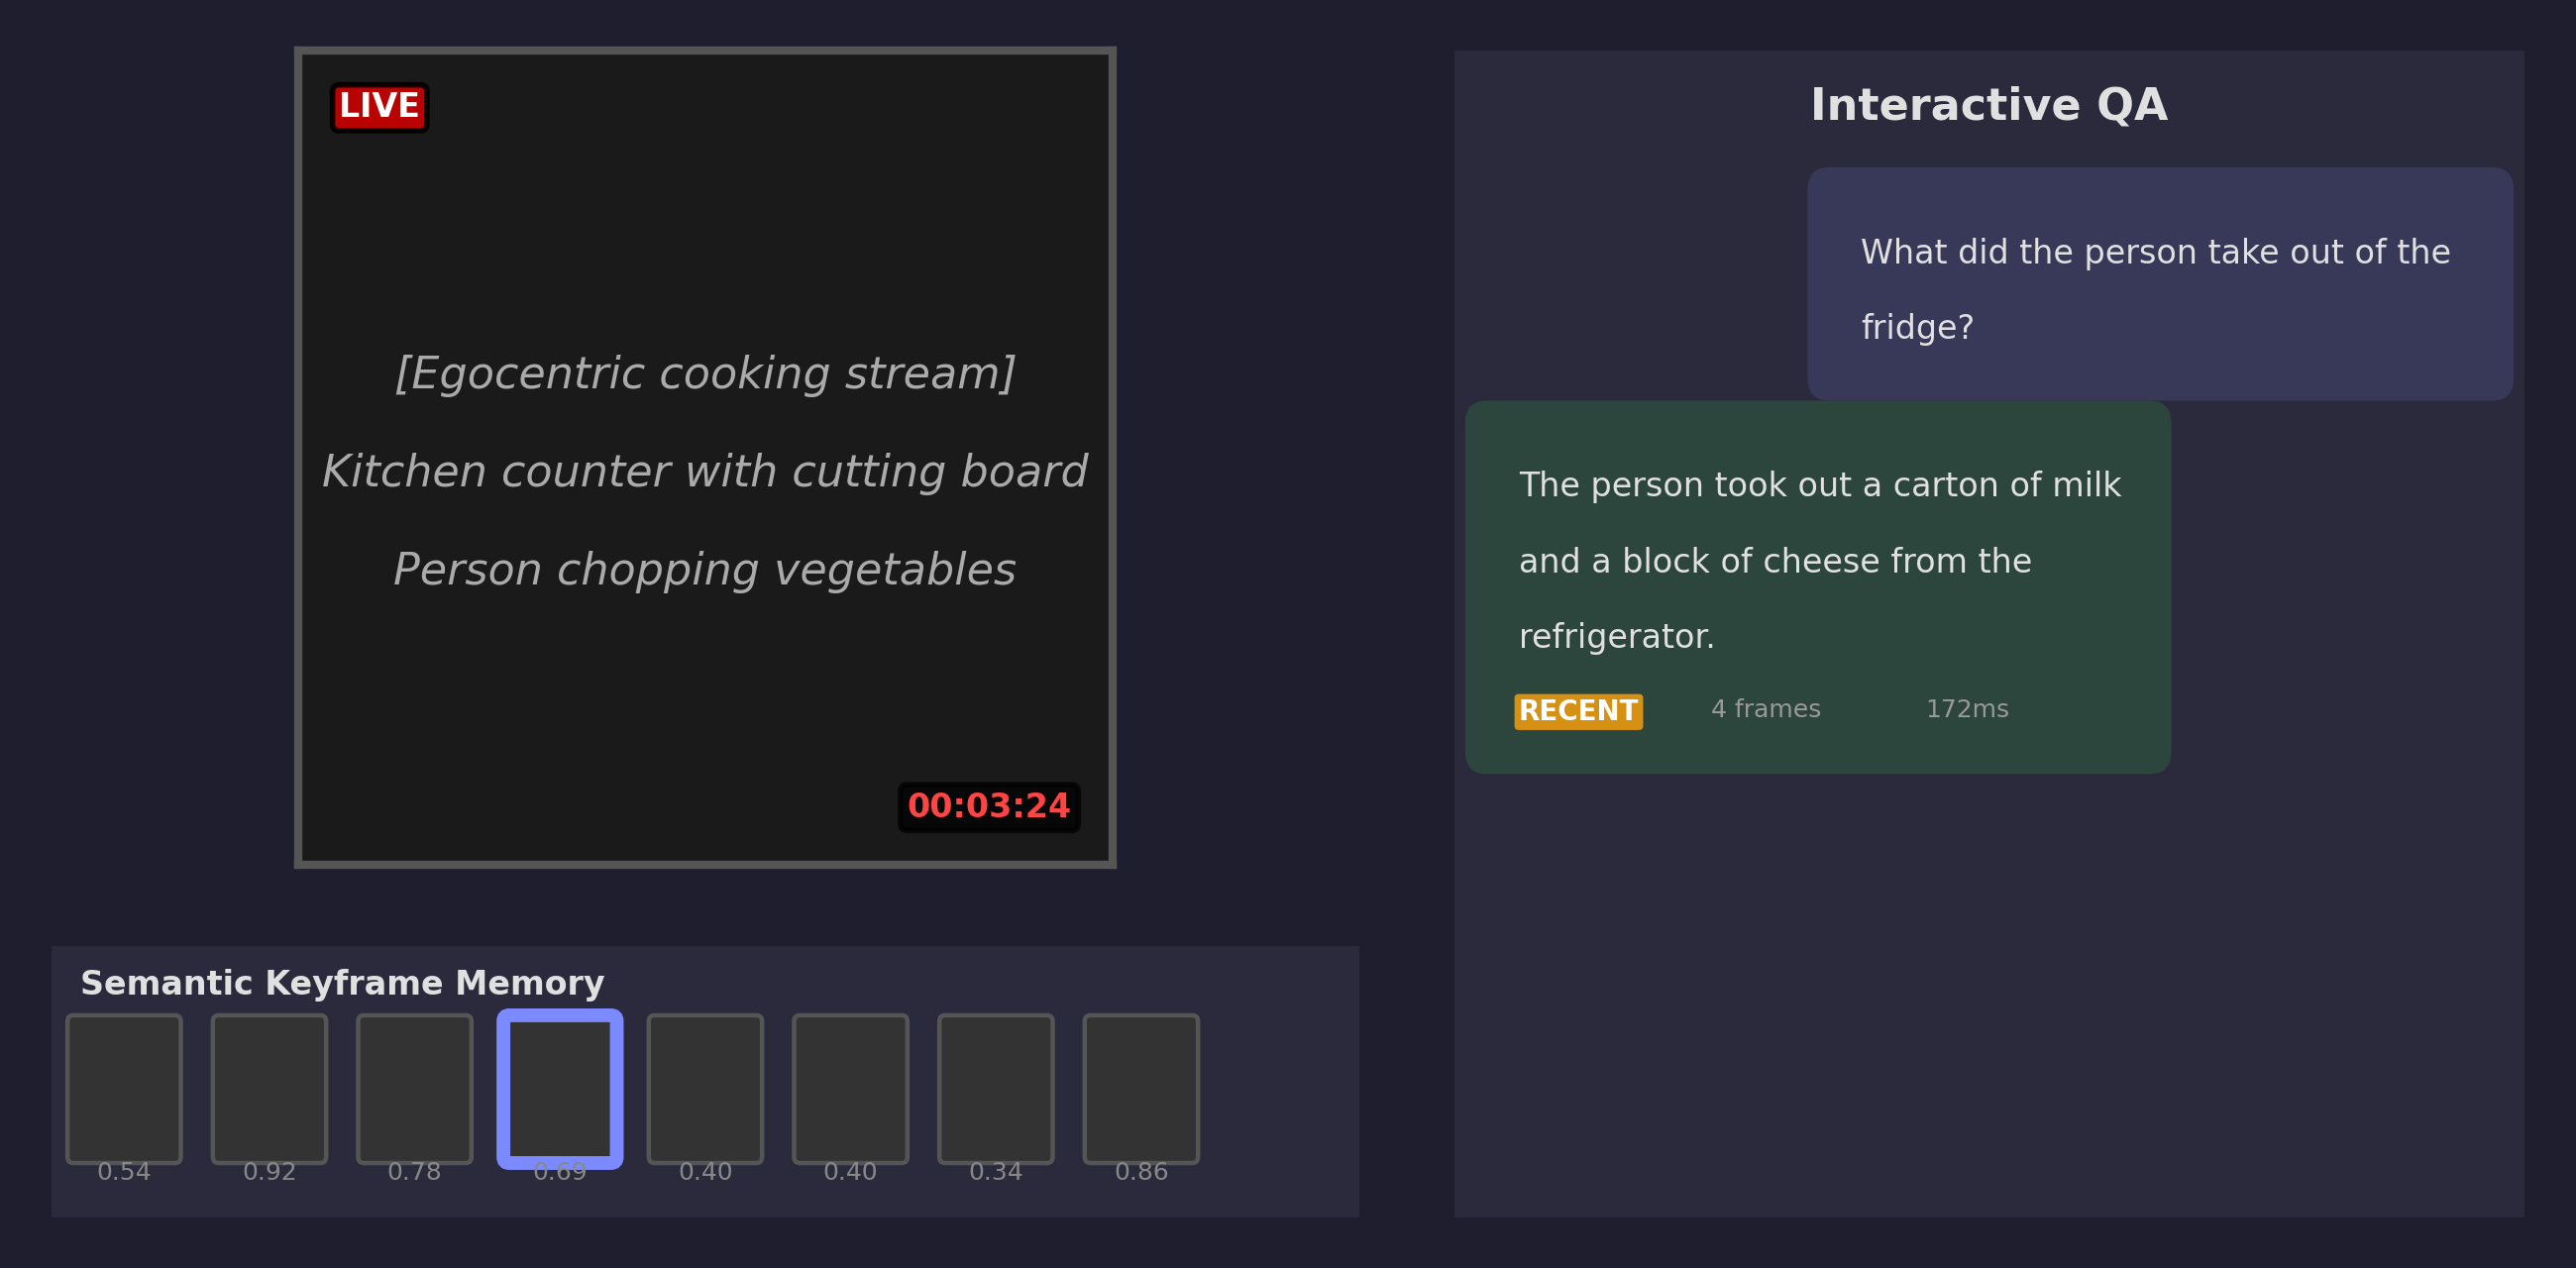
\includegraphics[width=\linewidth]{figures/qual_recent.pdf}
    \caption{Recent-scope query on a cooking stream.}
    \label{fig:qual-recent}
  \end{subfigure}
  \hfill
  \begin{subfigure}{0.32\linewidth}
    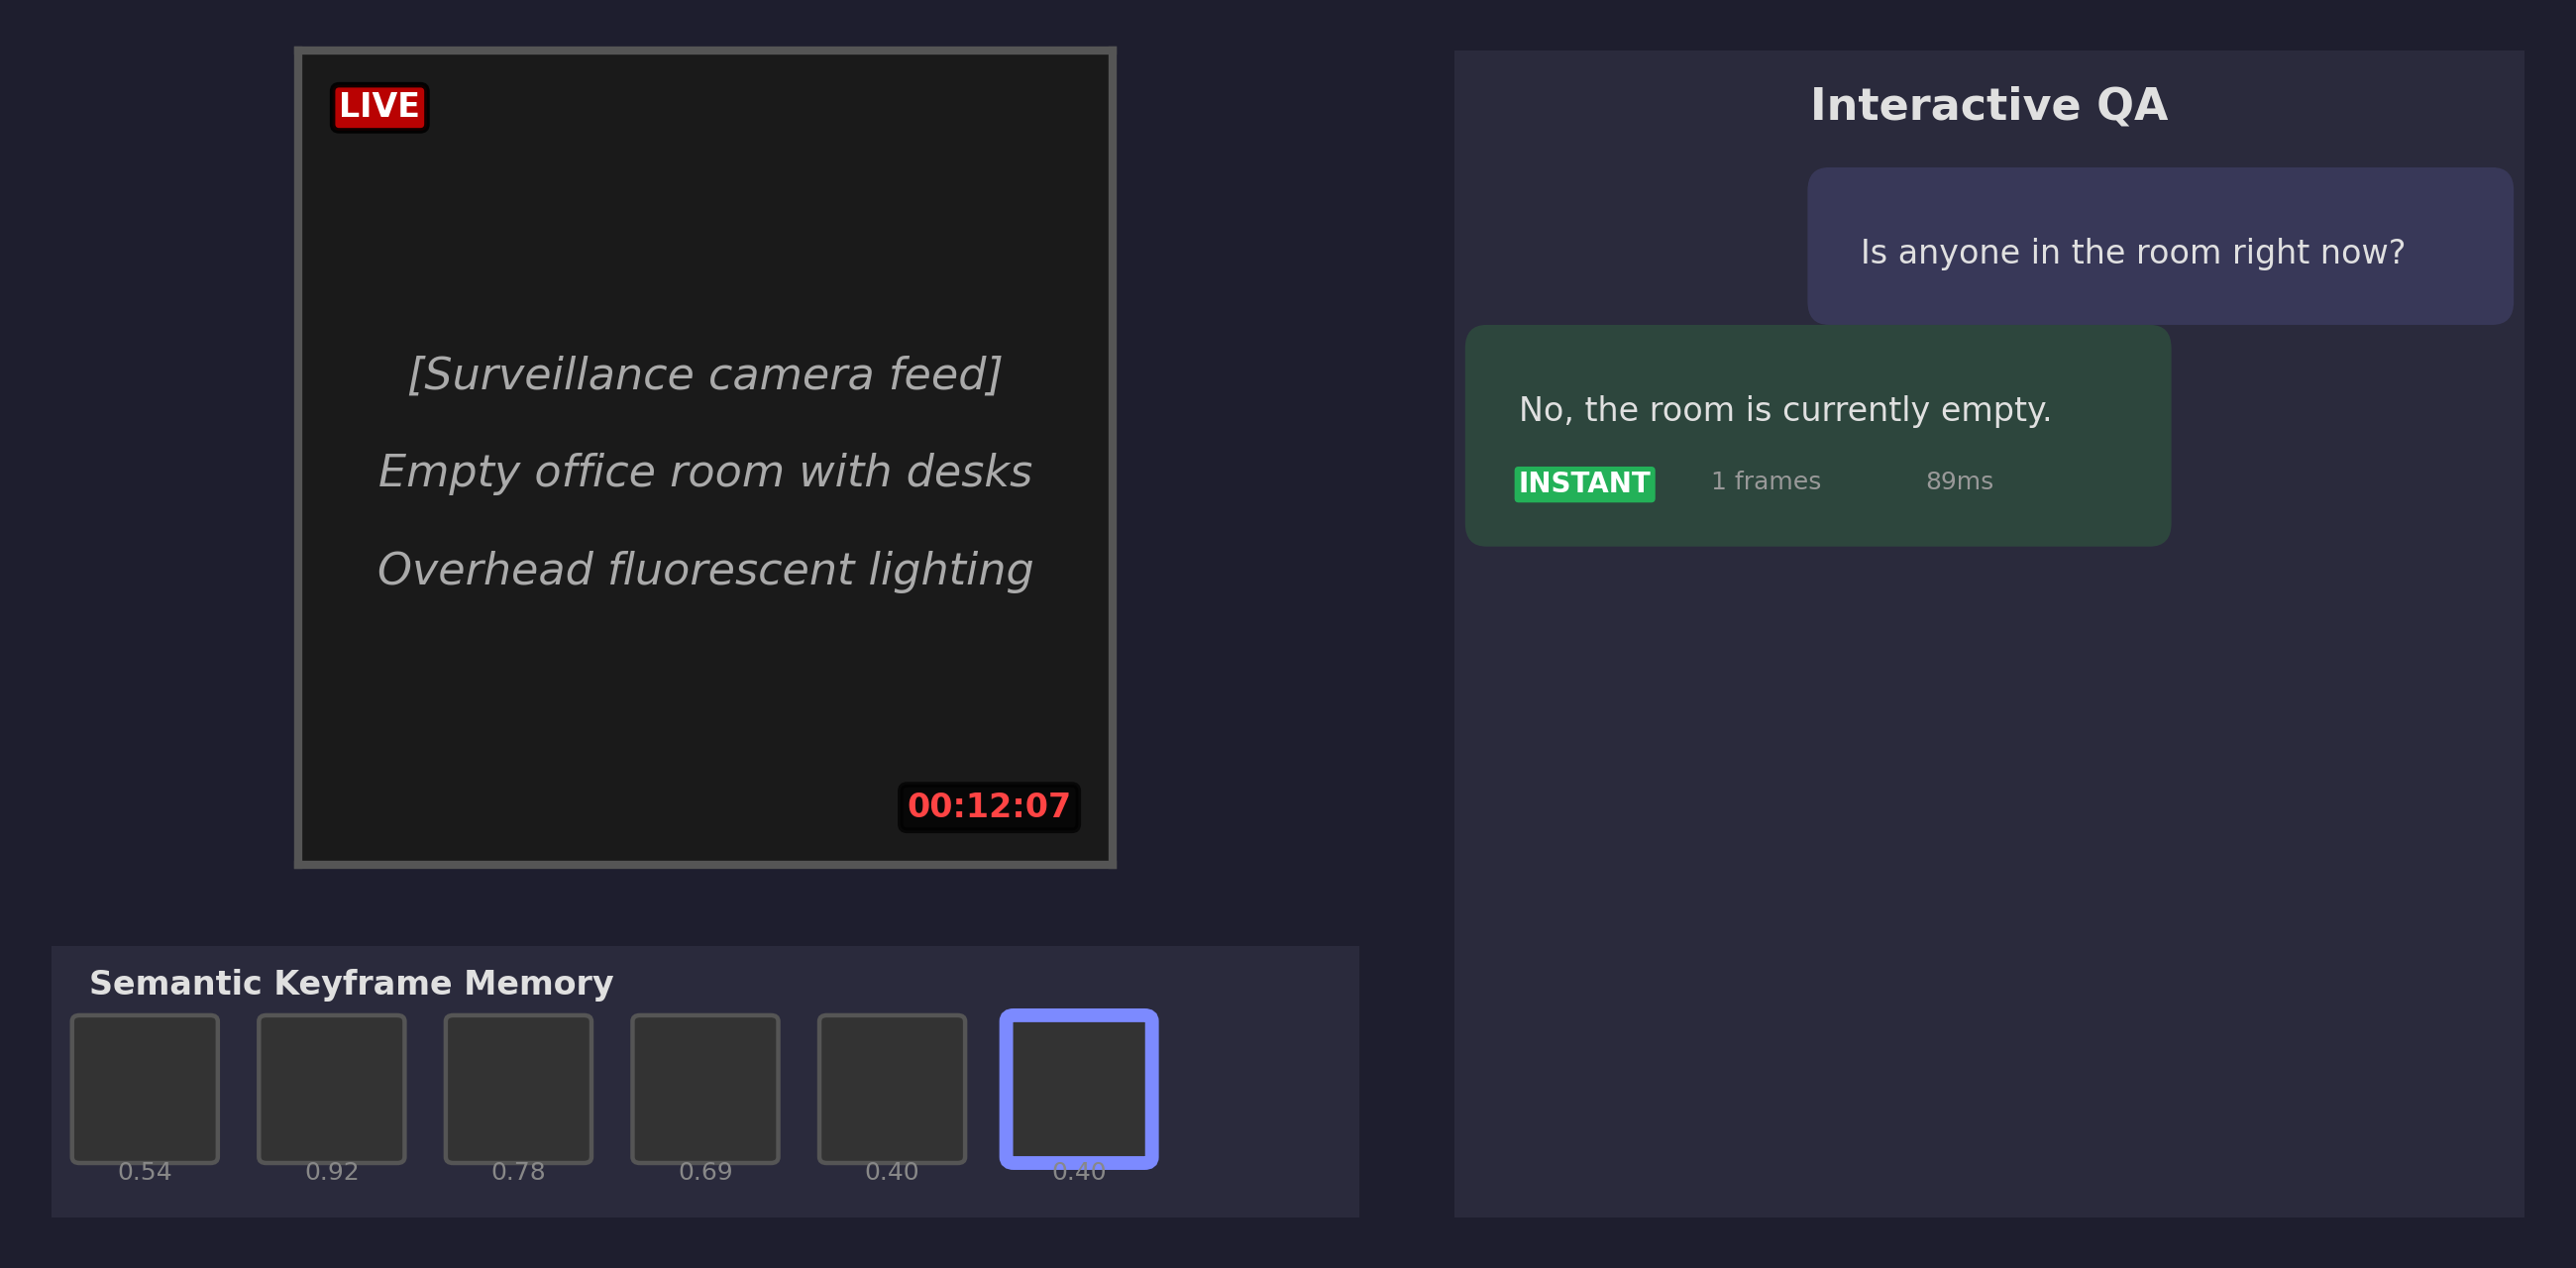
\includegraphics[width=\linewidth]{figures/qual_instant.pdf}
    \caption{Instant-scope query on a surveillance feed.}
    \label{fig:qual-instant}
  \end{subfigure}
  \hfill
  \begin{subfigure}{0.32\linewidth}
    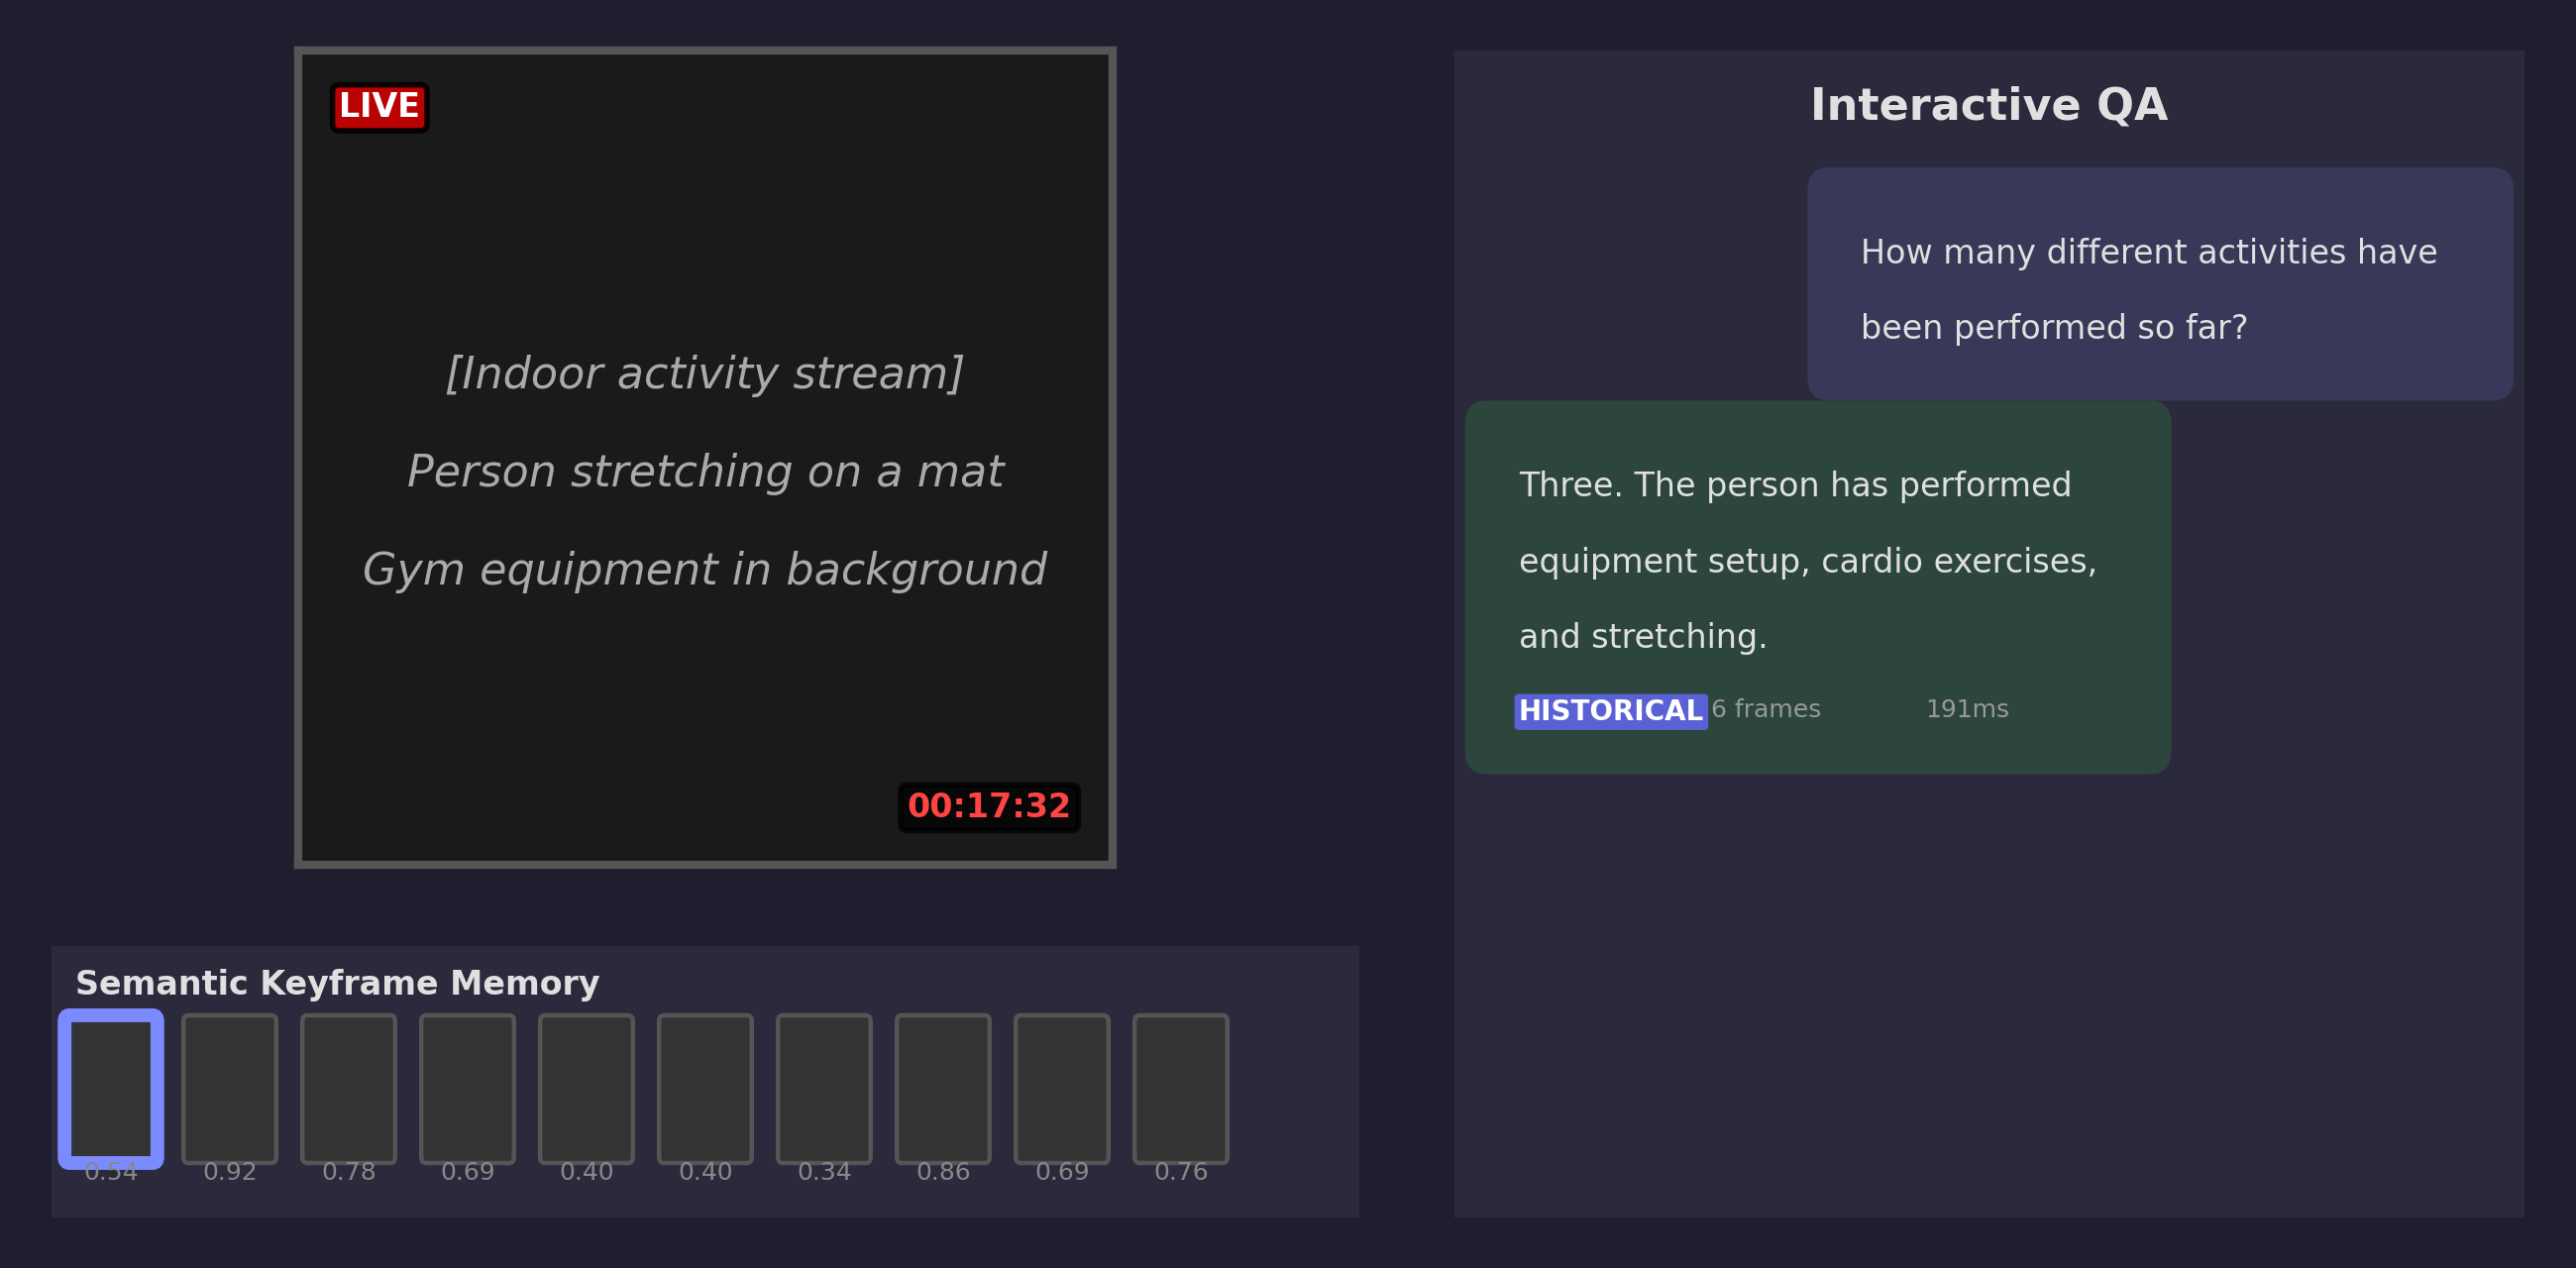
\includegraphics[width=\linewidth]{figures/qual_historical.pdf}
    \caption{Historical-scope query on an activity stream.}
    \label{fig:qual-historical}
  \end{subfigure}
  \caption{\textbf{Qualitative examples.} Three representative queries spanning all temporal scopes. Each panel shows the live video frame (top-left), SKM filmstrip (bottom-left), and the Q\&A interaction with scope tag and latency (right). \ours routes each question to the correct time window and produces grounded answers.}
  \label{fig:qualitative}
\end{figure*}

\subsection{Qualitative Results}
\label{sec:qualitative}

\Cref{fig:qualitative} shows three demo queries, one per scope.
In~(a), \emph{``What did the person take out of the fridge?''} triggers \textsc{recent}; the SKM retrieves the last 30\,s of keyframes and the answer correctly identifies \emph{milk and cheese}.
In~(b), \emph{``Is anyone in the room right now?''} triggers \textsc{instant}; only the latest frame is used and the system answers \emph{``No, the room is currently empty.''}
In~(c), \emph{``How many different activities have been performed so far?''} triggers \textsc{historical} over a 15-minute stream. BLIP captions across 64 keyframes reveal three distinct activities; a FIFO buffer would have overwritten the early frames.

\paragraph{LiveQA-Bench examples.}
\Cref{fig:liveqa_examples} shows two additional LiveQA-Bench predictions.
A \textsc{historical} query on a 12-minute home stream (\emph{``Did anyone leave the room earlier?''}) correctly identifies a departure event retained as a high-novelty frame.
A \textsc{recent} query on a 20-minute kitchen stream (\emph{``What was just placed on the counter?''}) retrieves the last 30\,s and identifies a cutting board and vegetables.

\begin{figure}[t]
  \centering
  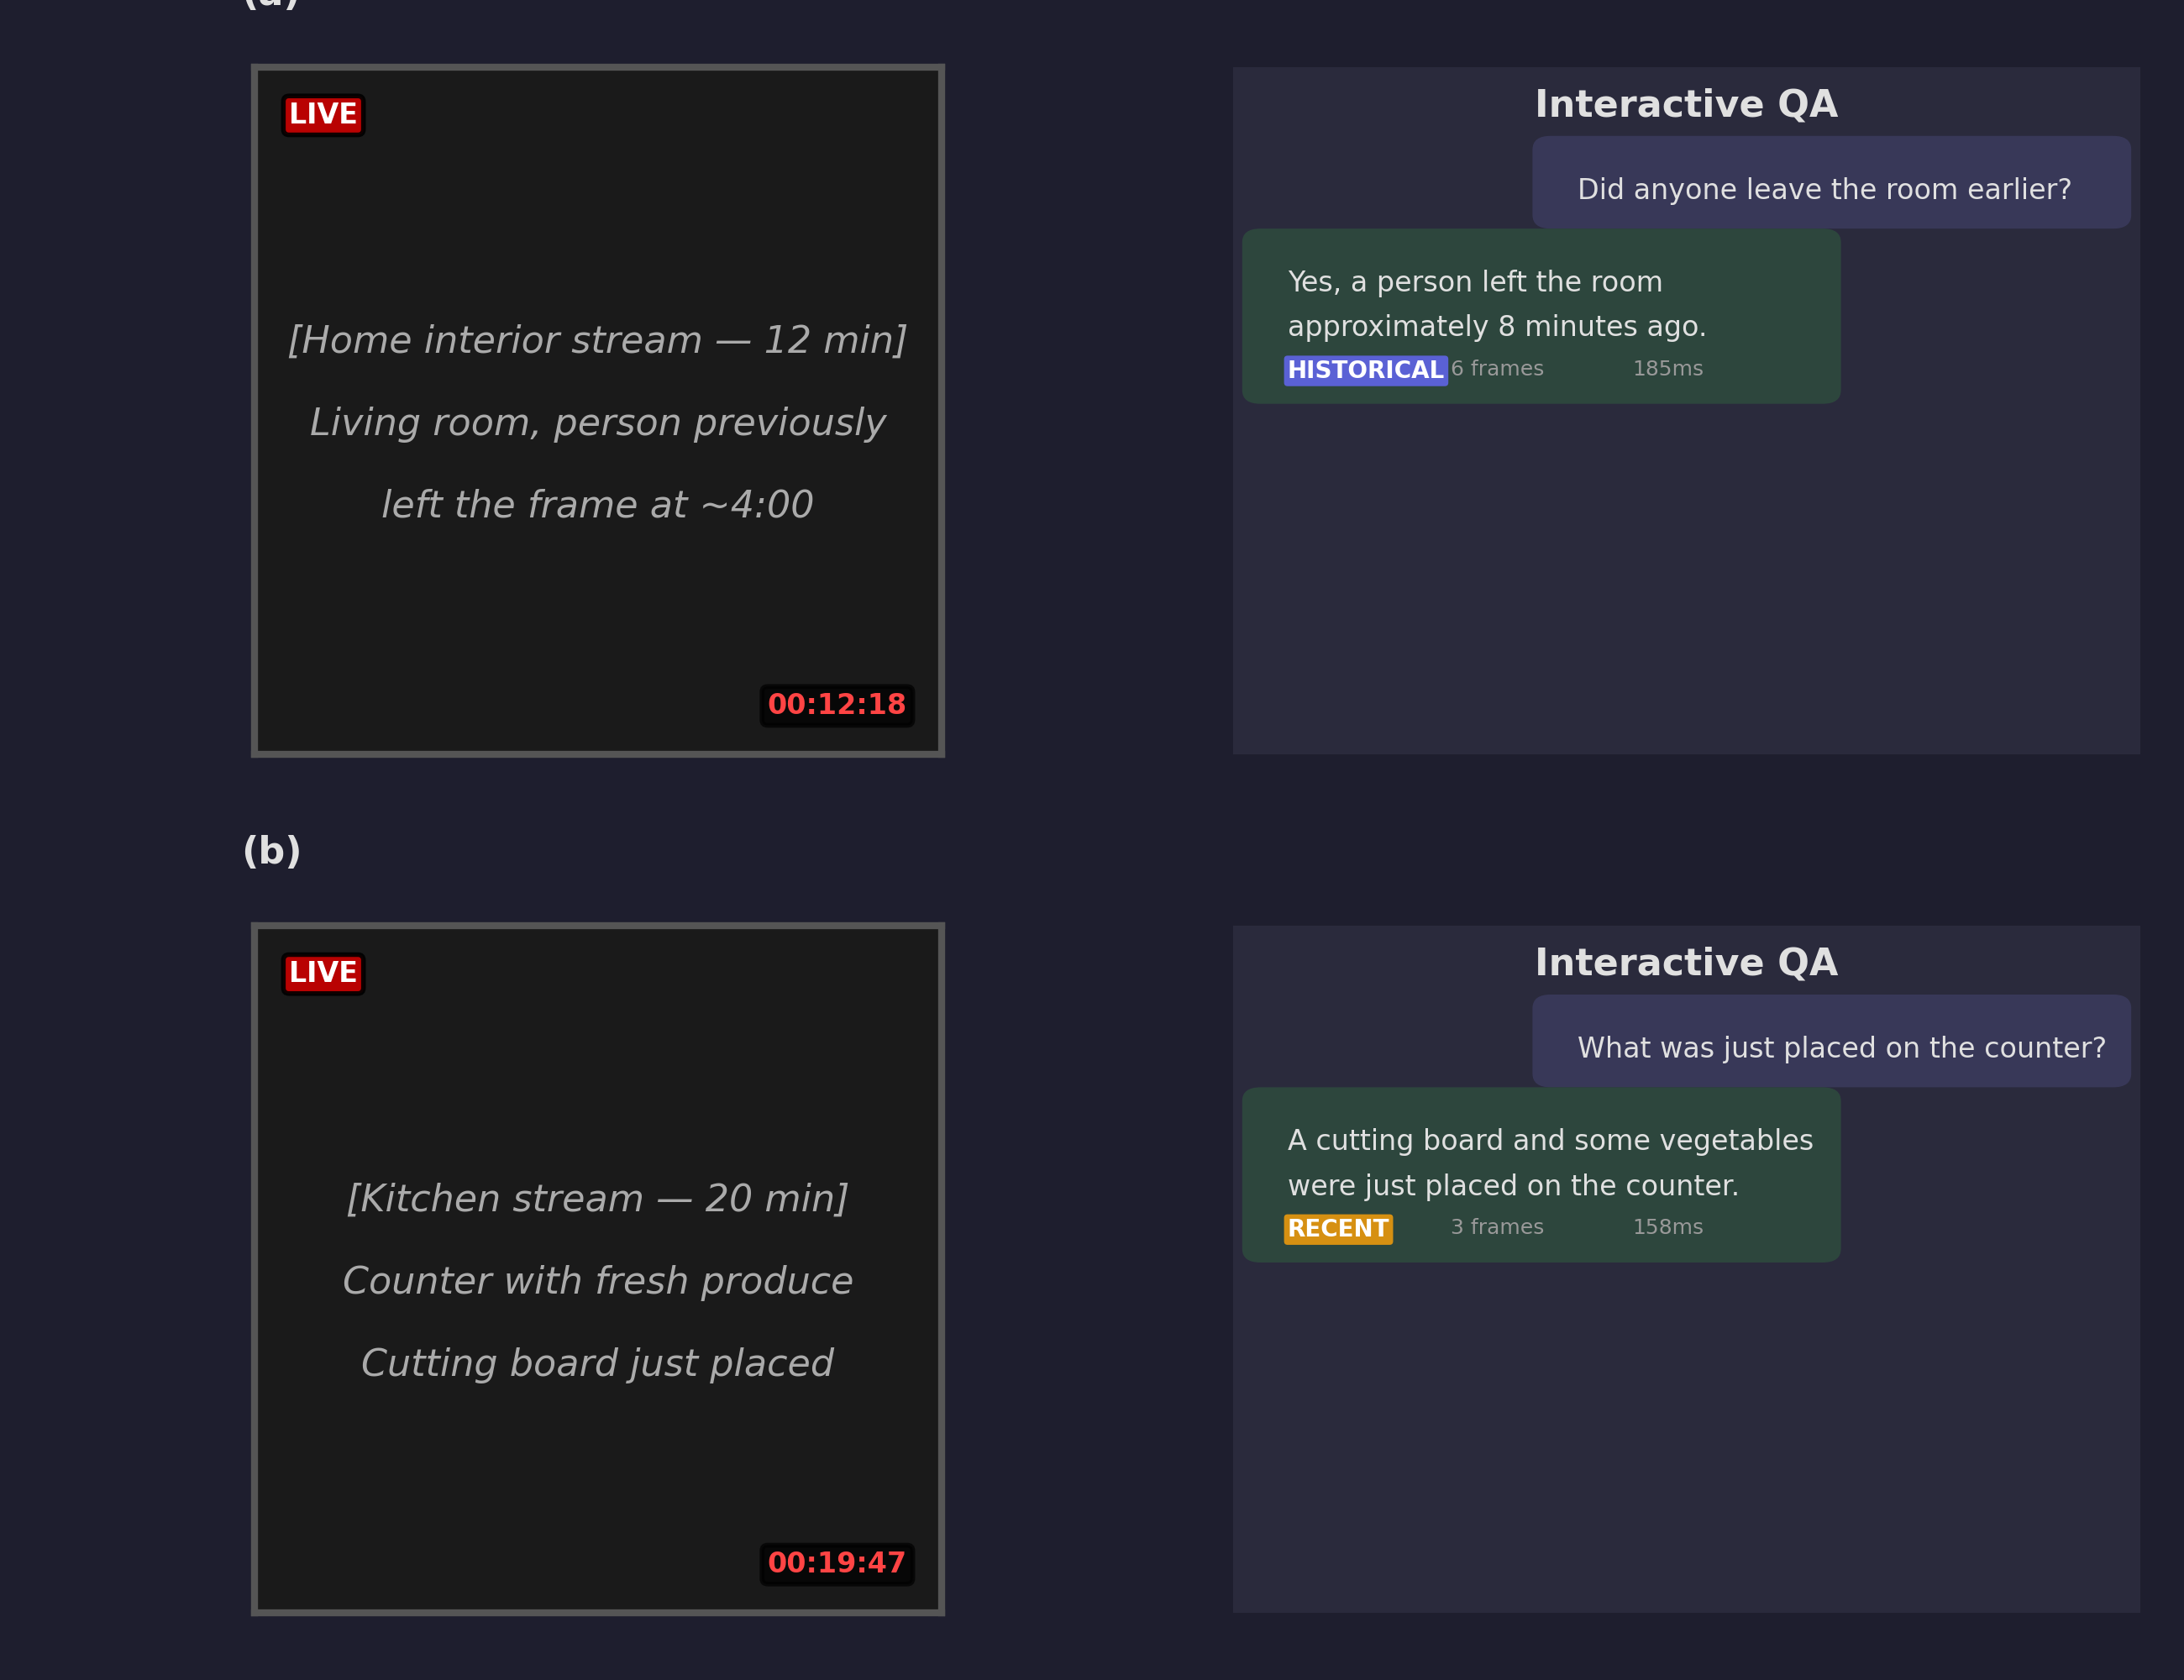
\includegraphics[width=\linewidth]{figures/qual_liveqa_examples.pdf}
  \caption{\textbf{LiveQA-Bench predictions.} Two examples showing historical (top) and recent (bottom) scope routing on long simulated streams. Correct scope classification enables accurate answers even for events that occurred minutes earlier.}
  \label{fig:liveqa_examples}
\end{figure}
